\subsection*{(i)}

Using Lebniz' rule we obtain af ordinary backward differential equation for the reserve $\tilde V_0$. We have

\begin{align*}
\frac{d}{dt}\tilde V_0(t)
&= \int_t^{\infty} \frac{\partial}{\partial t}
e^{-\int_t^s (\tilde r(u) + \tilde \mu(u))\,du} \, ds -1  \\
&= \int_t^{\infty}
e^{-\int_t^s (\tilde r(w) + \tilde \mu(w))\,dw}
(\tilde r(t) + \tilde \mu(t))\, ds -1 \\ 
&=(\tilde r(t) + \tilde \mu(t))
\int_t^{\infty}
e^{-\int_t^s (\tilde r(w) + \tilde \mu(w))\,dw} \, ds - 1 \\
&= (\tilde r(t) + \tilde \mu(t)) \tilde V_0(t) - 1,
\end{align*}

with $\tilde V_0(111)=0$.

Now, using the fourth order Runge-Kutta method we optain a numerical solution of $\tilde V_0(t)$. The result is shown via the plot below

\begin{figure}[h]
    \centering
    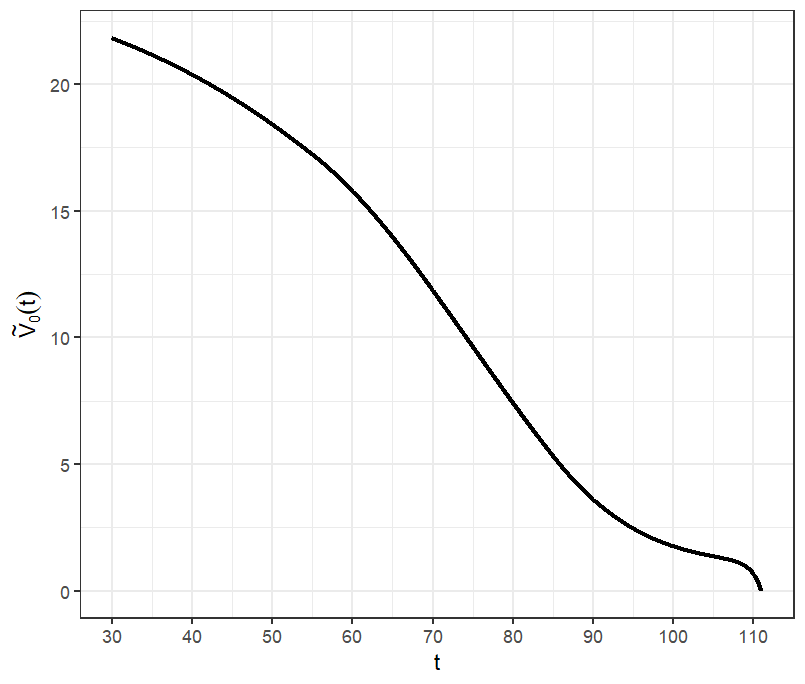
\includegraphics[width=0.5\linewidth]{Pictures/tildeV_0.png}
\end{figure}